\documentclass[aps,letterpaper,11pt]{revtex4}


\usepackage{graphicx} % For images
\usepackage{float}    % For tables and other floats
\usepackage{verbatim} % For comments and other
\usepackage{amssymb}  % For more math
\usepackage{fullpage} % Set margins and place page numbers at bottom center
\usepackage{listings} % For source code
\usepackage[usenames,dvipsnames]{color} % For colors and names
\usepackage[pdftex]{hyperref}           % For hyperlinks and indexing the PDF
\usepackage{pdfpages}
\usepackage{subfig}

\usepackage{listings}
\usepackage[usenames,dvipsnames,svgnames,table]{xcolor}
\usepackage{color}
\usepackage{textcomp}
\usepackage[utf8]{inputenc}

% Default fixed font does not support bold face
\DeclareFixedFont{\ttb}{T1}{txtt}{bx}{n}{12} % for bold
\DeclareFixedFont{\ttm}{T1}{txtt}{m}{n}{12}  % for normal

% Custom colors
\definecolor{deepblue}{rgb}{0,0,0.5}
\definecolor{deepred}{rgb}{0.6,0,0}
\definecolor{deepgreen}{rgb}{0,0.5,0}

% Python style for highlighting
\newcommand\pythonstyle{\lstset{
language=Python,
basicstyle=\ttm,
otherkeywords={self},             % Add keywords here
keywordstyle=\ttb\color{deepblue},
breaklines=true,
emph={MyClass,__init__},          % Custom highlighting
emphstyle=\ttb\color{deepred},    % Custom highlighting style
stringstyle=\color{deepgreen},
frame=tb,                         % Any extra options here
showstringspaces=false            % 
}}

\newcommand\launchstyle{\lstset{
    language=xml,
    tabsize=3,
    %frame=lines,
    frame=tb,
    rulesepcolor=\color{gray},
    xleftmargin=20pt,
    framexleftmargin=15pt,
    otherkeywords={node,include,param},
    keywordstyle=\ttb\color{deepblue},
    commentstyle=\color{orange},
    stringstyle=\color{deepgreen},
    breaklines=true,
    showstringspaces=false,
    basicstyle=\ttm,
    emph={pkg,args,value,file,name,type},
    emphstyle={\color{deepred}}}
    }


% Python environment
\lstnewenvironment{python}[1][]
{
\pythonstyle
\lstset{#1}
}
{}



% Launch for external files
\newcommand\pythonexternal[2][]{{
\pythonstyle
\lstinputlisting[#1]{#2}}}

% Python for external files
\newcommand\launchexternal[2][]{{
\launchstyle
\lstinputlisting[#1]{#2}}}

% Python for inline
\newcommand\launchstyleinline[1]{{\launchstyle\lstinline!#1!}}

\newcommand\pythoninline[1]{{\pythonstyle\lstinline!#1!}}
 
\hypersetup{ % play with the different link colors here
    colorlinks,
    citecolor=black,
    filecolor=black,
    linkcolor=black,
    urlcolor=blue % set to black to prevent printing blue links
}

\newcommand{\labno}{Technical report}
\newcommand{\labtitle}{Motion Control on TurtleBot}
\newcommand{\authorname}{Kevin Descharrieres, Antoine Merlet}
\newcommand{\professor}{Dr. Ralph Seulin}






\begin{document}  
\begin{titlepage}
\begin{center}
{\LARGE \textsc{\labno:} \\ \vspace{4pt}}
{\Large \textsc{\labtitle} \\ \vspace{4pt}} 
\rule[13pt]{\textwidth}{1pt} \\ \vspace{150pt}
{\large By: \authorname \\ \vspace{10pt}
Professor: \professor \\ \vspace{10pt}
\today}
\end{center}




\end{titlepage}% END TITLE PAGE %%%%%%%%%%%%%%%%%%%%%%%%%%%%%%%%%%
\newpage
\tableofcontents
\newpage

\section{Presentation of the robot}

\begin{figure}[H]
	\centering
	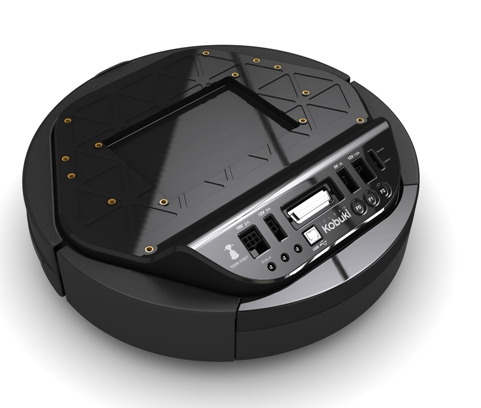
\includegraphics[height=8cm]{Mobile-Robot-Kobuki.jpg}
	\caption{Kobuki Base}
	\label{fig:Robot Base}    
\end{figure}

The first version of the TurtleBot was created in 2011 by Willow Garage society. This robot hardware, based on a vacuum cleaner, has been improved over the time and is now considered as a pillar of the robotic field. The aim of this robot is to make it affordable for a beginner in the field while being powerful enough for high-end applications. Moreover, the TurtleBot OS is based on the middle-ware ROS (Robot Operating System), making it a really nice tool as ROS is becoming more and more popular. By now, the TurtleBot became THE reference in education and research.

As any first version of a hardware/software, the TurtleBot could be improved, giving therefore the TurtleBot 2 (the one we are equipped with). Following are presented the main features of this robot:

\begin{itemize}
\item {A comfortable operating time (2-3 hours);}
\item {A Kinect for 3D sensing;}
\item {A fast charging Dock for idling charge;}
\item {A charging cable in order to charge the base while using it;}
\item {Cliff and drop sensors;}
\item {A laptop;}
\item {And 3 collision sensors.}
\end{itemize}

\begin{figure}[H]
	\centering
	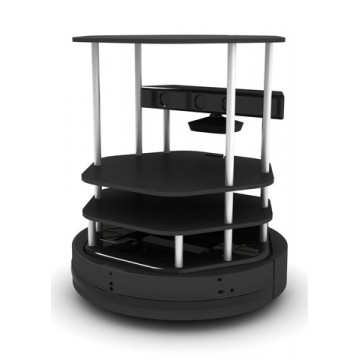
\includegraphics[height=8cm]{turtlebot-2-robot-mobile-ros.jpg}
	\caption{TurtleBot 2}
	\label{fig:Robot Components}    
\end{figure}

For more technical details about the Kobuki base, please refer to [1] (link it to the doc). Most all the work has been done using a very complete book: ROS by example, volume 1, R. Patrick Goebel.


\section{How to control a TurtleBot}
\subsection{Workspace and network}
There are mainly two ways of controlling the TurtleBot. 
The first option is to directly control the TurtleBot using the laptop connected to it. However, this is inconvenient as the TurtleBot might be moving, but also because the user does not have any comfortable position to use the laptop.

The second option is to remotely connect to the TurtleBot computer. This can be easily done with Ubuntu by using the SSH build-in command. Also, please notice that the network is already optimized in our case (singleton of the couple Workspace+TurtleBot per router), making the SSH really easy on our side. Therefore, you can distinguish two main components: the TurtleBot+laptop and the Workstation. This allows the control of the TurtleBot in an efficient (and comfortable) way. The only thing that is to be done to enable the remote control is to modify the bashrc file of the workstation (located in the Home folder in most of the cases, can be edited by using the command \textit{\$ gedit {\raise.17ex\hbox{$\scriptstyle\sim$}} /.bashrc}. The three last lines ('export') need to be uncommented. The first one should contain the IP address of the TurtleBot on your local network (most-likely starting by 192.168.XXX.XXX). The two second line should be filled with the IP of your Workstation. In order to make it easy for daily connection, we suggest that both the Workstation and the TurtleBot laptop are provided static IP addresses. 

In all the following, we will specify one which one should be started each command line. If not specified, the main computer (the workstation) should be considered as the default one. If you would like to see our workstation organization for a simple application, please check out \href{https://www.youtube.com/watch?v=OgMLn4ib6k8}{this video}.

\subsection{Topics and nodes}

A node represent a process, doing calculations. With ROS, each node is dedicated to a specific take. For example, one node manages the lidar, another on the Kinect, one the movement of the wheels, and so on. In order to communicate, Nodes are using Topics, by publishing messages into it. This topic has a specific name representing the type of data that it is carrying (the topic "joy" carries information about the joystick input). Node are not only publishing to topics, they can also subscribe to them, so that when a new topic publishes, they receive this data. This concepts are simple as long as the application is basic, otherwise, it is really complicated to figure out which node is publishing to which topic. In order to have a price idea of what is going on at a low level, a very powerful tool can be used: the rqt\_graph (presented later).

\subsection{Package}

A way to control the TurtleBot is to create a package. This allows to store several behaviours for the TurtleBot. In order to create such a package, one could either use the command 
\textit{\$ catkin\_create\_pkg \textless package \_name\textgreater [depend1] [depend2] [depend3]} by replacing the given parameters by the wanted name and dependencies. It is also possible to create manually a package from scratch, mostly for advanced users with a wide knowledge of ROS. In our case, we used the command \textit{\$ catkin\_create\_pkg project rospy std\_msgs}. Therefore, the package is named 'project' and is using two external libraries. Rospy is used to be able to create and run python scripts with the TurtleBot, and std\_msgs allowing to use standard data-types. The package also comes with a file named 'CMakeLists.txt', which we are not changing. The package also comes along with folders, such a scripts and launch files.

\subsection{Script}

In order to create your own routines for the robot, Scripts are used. They are mainly written in Python or C++ language, which are widely used in IT science, making it somewhat easy to create. Following is presented the basic commands to create a Python script for ROS.


\begin{python}
# Always import rospy for the script to work
import rospy

# Initializing a Self-created node called MyNode
rospy.init_node('MyNode')

# Declaring a new publisher to the Topic /cmd_vel. 
self.cmd_vel = rospy.Publisher('/cmd_vel', Twist, queue_size=1)
	
# Initialize the movement command that will be emitted to the publisher
move_cmd = Twist()

# Publishing the move_cmd message to the publisher (being /cmd_vel)
self.cmd_vel.publish(move_cmd)

# Putting the robot in sleep mode (usually when the script is done)
rospy.sleep(1)
\end{python}

Once the TurtleBot is started with a ROScore, it is possible to start scripts. However, having to start the ROScore with all the scripts needed for the experiment can be a bit tedious. Launch files can overcome this problem.

\subsection{Launch files}
Script file are simple to use, but not very convenient. Launch files bring the possibility to start several scripts and launch file as well as allowing to use custom settings. The following example show all of this.
\launchexternal{class_joy2twist.launch}
As we can see on the first few lines, this launch file is starting another launch file. This included file may or may not include again other launch files, et caetera. From this, we can obviously see a big source of problem: any time you there is a need to debug one application, all launch files must be examined recursively. It is not unusual to have around seven layers of launch file.
In the launch files, it is also possible to set the values of parameters from the included nodes. Finally, it is also possible to remap some topics, transferring the published data to another topic.

\subsection{Bag files}
ROS is equipped with a very powerful to record all the topics and nodes while the robot is processing them: the bag files. This files can then be replayed, either in simulation or on a real robot, by publishing the topics in the bag file. For this project, we recorded each of our script running on a robot.



\section{Our project}
\subsection{Purpose}
The main goal of this project is to learn ROS buy producing code to control the TurtleBot. The last part of the project is an innovation part: we will try to ROSify the PhantomX Arm Pincher, from TrossenRobotics.
As a support fr the project, we used three main source of information: the ROS online documentation, the lessons given by our professors and the ROS by example book. 
In order to start the project,  created a package, wisely called `project' for the time beeing. As we are beginners in the field, we did not change the CMakeLists file, and included only the basic libraries in our project.

\subsection{Simple motions, Twist and Odometry
}\begin{figure}[H]
	\centering
	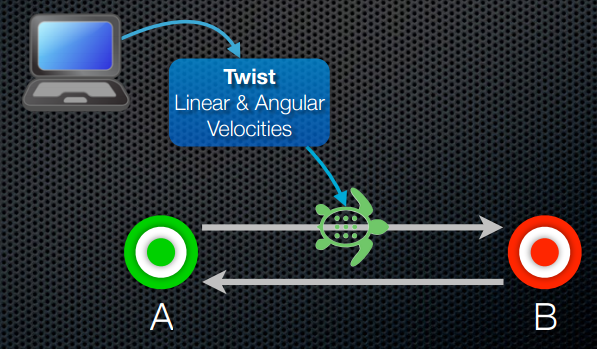
\includegraphics[height=8cm]{come-and-back.png}
	\caption{Come and Back movement}
	\label{fig: Come and Back movement}    
\end{figure}
The very first step to perform in order to control the TurtleBot is to implement methods for the basic movement: moving forward. As the code for this very first part is given in the ROS by example, we used it as the first stone of our project. In fact, we did spend time to understand the structure of the file. 
From the lessons, we know thata  twist message can be used to move the robot, and we also know that a Publiser is needed to send this message to the TurtleBot. We know that a Twist message takes as parameter a linear velocity as well as an angular velocity. At this point, the system is in an open loot, and we can not have any feedback on the robot position. We will therefore set the goal distance at 1 meter, and perform in the script calculations to estimate the time needed to move to the goal, given the linear speed of the robot ( 0.2 meter per second in our case, for safety matters). Once the movement is performed, a 180° rotation is needed to turn around. In this part, we need to define an angular velocity, and perform computations again to have an estimation of the time needed for the rotation. By placing these two parts, moving forward and rotate, in a for loop perfomed twice we should the be able to perform the back and forth. Following is presented the code corresponding to the previous descritpion: 
\begin{python}
#!/usr/bin/env python

import rospy
from geometry_msgs.msg import Twist
from math import pi

class BackAndForth():
    def __init__(self):
        # Init the node. Not anonymous cbecause only one 
        rospy.init_node('back_and_forth', anonymous=False)

        # When shutdown, perfoms launch the shutdown function below      
        rospy.on_shutdown(self.shutdown)
        
        # This is the publisher to the cmd_vel
        self.cmd_vel = rospy.Publisher('/cmd_vel', Twist, queue_size=1)
        
        # Frequency
        rate = 50
        r = rospy.Rate(rate)
        
        # Set our variables in meters and radians
        linear_speed = 0.2
        goal_distance = 1.0
        angular_speed = 1.0
        goal_angle = pi*2
        
        # Travel time estimations
        linear_duration = goal_distance / linear_speed
        angular_duration = goal_angle / angular_speed
        
        #Perfomed twice to have a back and forth
        for i in range(2):
            # Init the Twist message
            move_cmd = Twist()
            
            # Init the linear speed
            move_cmd.linear.x = linear_speed
            
            # Normalizing the travel duration according to the frequency
            ticks = int(linear_duration * rate)
            
            # Perform movement
            for t in range(ticks):
                self.cmd_vel.publish(move_cmd)
                r.sleep()
            
            # Stop the robot before the rotation
            move_cmd = Twist()
            self.cmd_vel.publish(move_cmd)
            rospy.sleep(1)
            
            # Init the angular speed
            move_cmd.angular.z = angular_speed

            # Normalizing the rotate duration according to the frequency
            ticks = int(goal_angle * rate)
            
            # Perform Rotation
            for t in range(ticks):           
                self.cmd_vel.publish(move_cmd)
                r.sleep()
                
            # Publish an empty message to stop the robot for a few moments before going back
            move_cmd = Twist()
            self.cmd_vel.publish(move_cmd)
            rospy.sleep(1)    
            
        # Back and forth finish, publishing empty message to stop the robot
        self.cmd_vel.publish(Twist())
        
    def shutdown(self):
        # Always stop the robot when shutting down the node.
        rospy.loginfo("Stopping the robot...")
        self.cmd_vel.publish(Twist())
        rospy.sleep(1)
 
if __name__ == '__main__':
    try:
        BackAndForth()
    except:
        rospy.loginfo("Back-and-Forth node terminated.")

\end{python}

Note: For the rest of the report we will mention only the important or new parts of each script. 

We tried it first in simulation mode, so that we do not crash the robot in a wall on the first day. The simulation gave the expected results. But when we tried it on the robot, nothing happended. We checked the Rqt\_graph, and the cmd\_vel node was active. In fact, we are publishing the twist message to the wrong place. The TurtleBot is equipped with a multiplexer on the cmd\_vel: cmd\_vel\_mux. This multiplexer is divided is several parts, such as teleop and navigation. All these parts have a priority order. This priorities are used to represent the impotance of a movement. If a message from a topic with a higher priority than the current one is published, then it will override the current routine. So we need to redirect our cmd\_vel to this multiplexer. To perfom such a thing, we used a very simple launch file: 

\launchexternal{back_and_forth.launch}

We see here that we are redirecting the cmd\_vel to cmd\_vel\_mux/input/teleop. All the future cmd\_vel messages wil be rediceted using launch files to the previously mentionned part of the mux.
In theory, this code should move the robot, and when done, the robot should be back at the starting position, facing the same direction. Below are presented the results : 
\begin{figure}[H]
    \centering
    \subfloat[Start]{{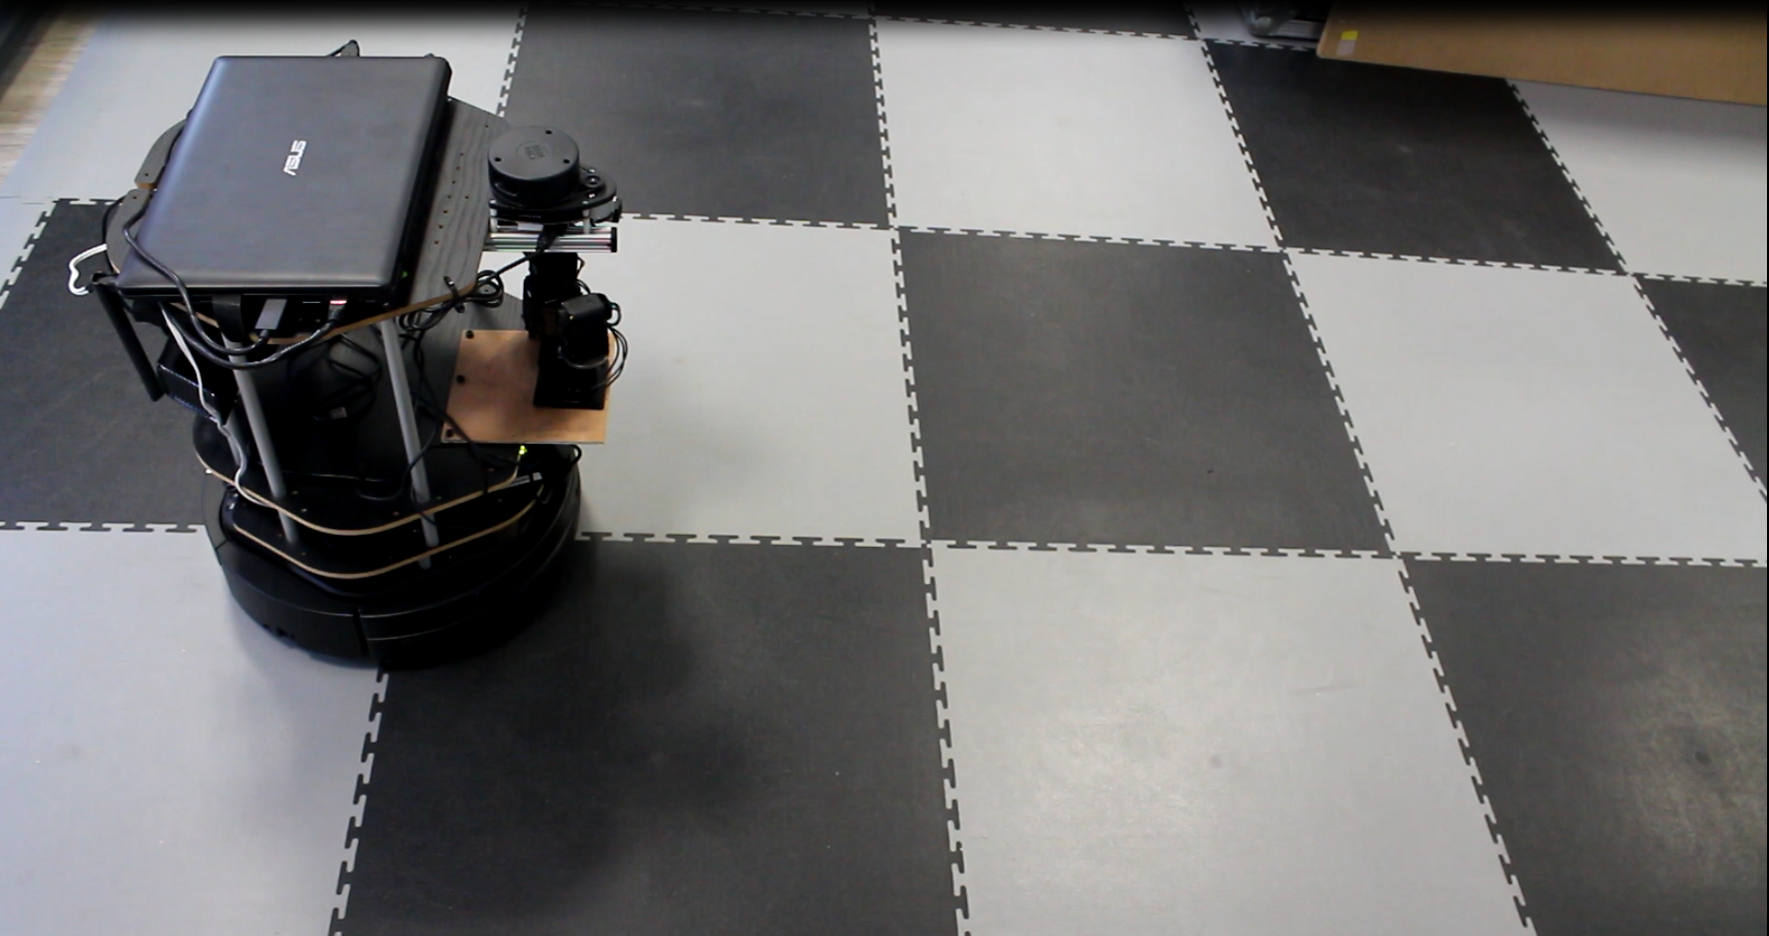
\includegraphics[width=7cm]{Back1.png} }}
    \qquad
    \subfloat[End]{{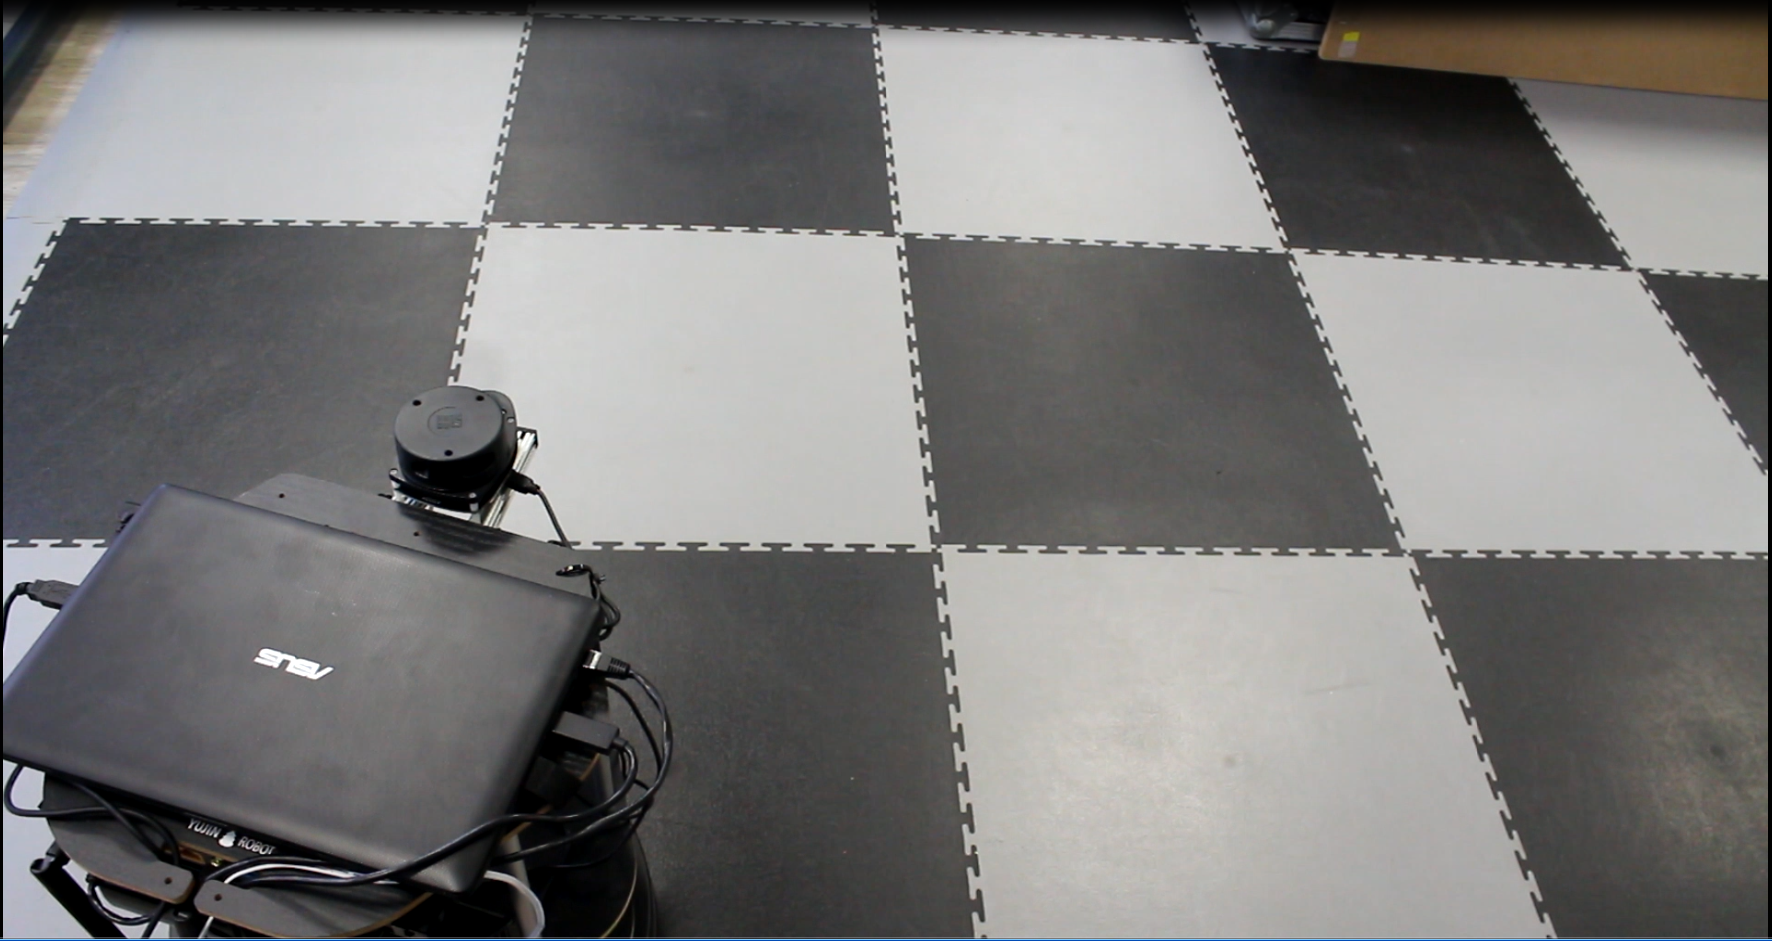
\includegraphics[width=7cm]{Back2.png} }}
    \caption{Comparision between starting and ending positions}
    \label{fig:example}%
\end{figure}

We can clearly see that the robot did not totally move as intended. This is due to the poor precision of the estimation. A robot can not be considered as working if it can not move in a straigth line. A closed-loop system with feedback on the position could be used to improve the precision. 
\begin{figure}[H]
	\centering
	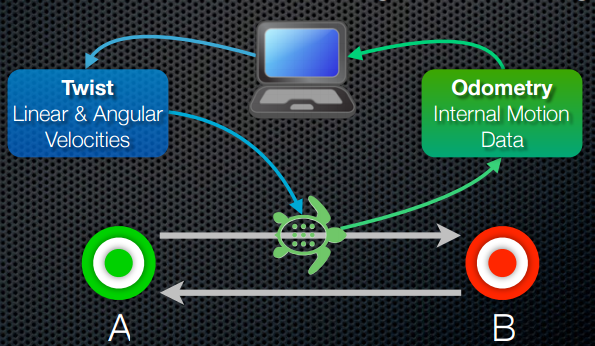
\includegraphics[height=8cm]{come-and-back-switch.png}
	\caption{Come and Back movement using odometry}
	\label{fig: Come and Back movement using odometry}    
\end{figure}
The robot's odometry could be used in order improve the precision. The first step to do this is to take in account a new reference frame: the odom frame. This frame is centered in the current robot position, therefore represented by (0,0,0). Then, each time that the robot moves, we retrive information from the odometry to compute the euclidian distance between the current position on the robot and the starting point. As soon as this euclidian distance is reach, the robot reaches the goal position, and is stop for few moemnts. On the same principle, we use the odometry to compute the roration of the robot. Below is presented the piece of code for the linear movement:

\begin{python}
	 # Init the total traveled distance
	 distance = 0
	 
            #Do as long as the goal is not reached
            while distance < goal_distance:
                # Publish the twist  previously set
                self.cmd_vel.publish(move_cmd)
                r.sleep()
        
                # Get the odometry
                (position, rotation) = self.get_odom()
                
                # Euclidian distance
                distance = sqrt(pow((position.x - x_start), 2) + 
                                pow((position.y - y_start), 2))
\end{python}

This method is giving totally different results, shown below: 

\begin{figure}[H]
    \centering
    \subfloat[Start]{{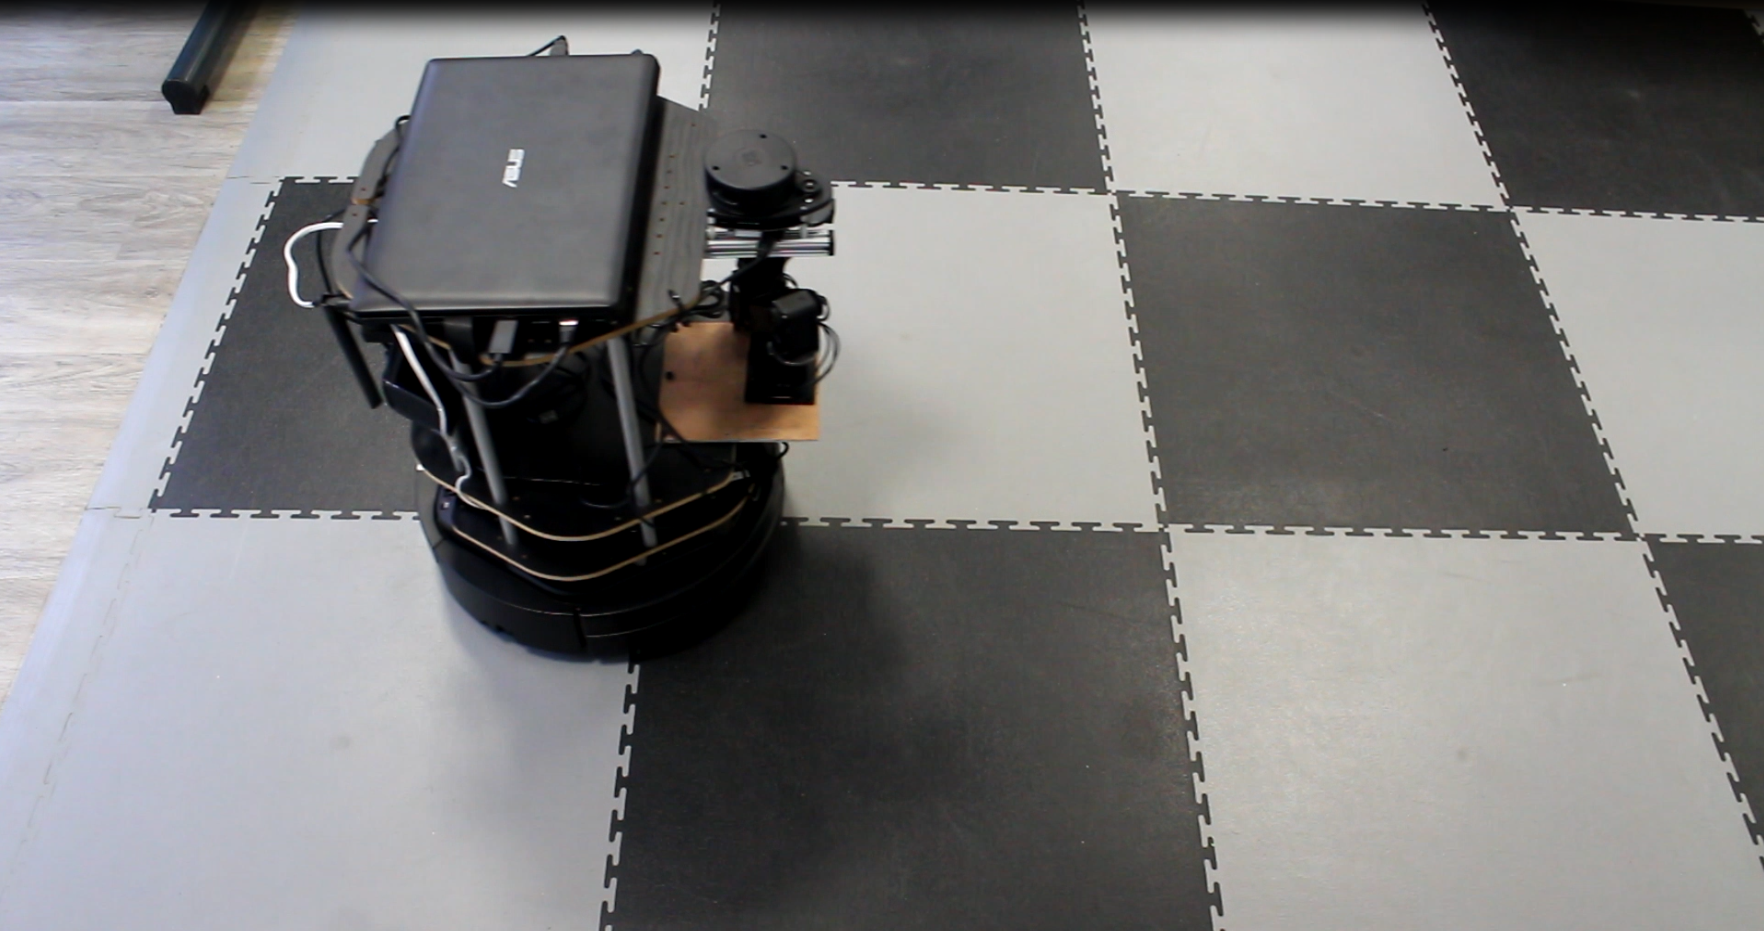
\includegraphics[width=7cm]{BackOdom1.png} }}
    \qquad
    \subfloat[End]{{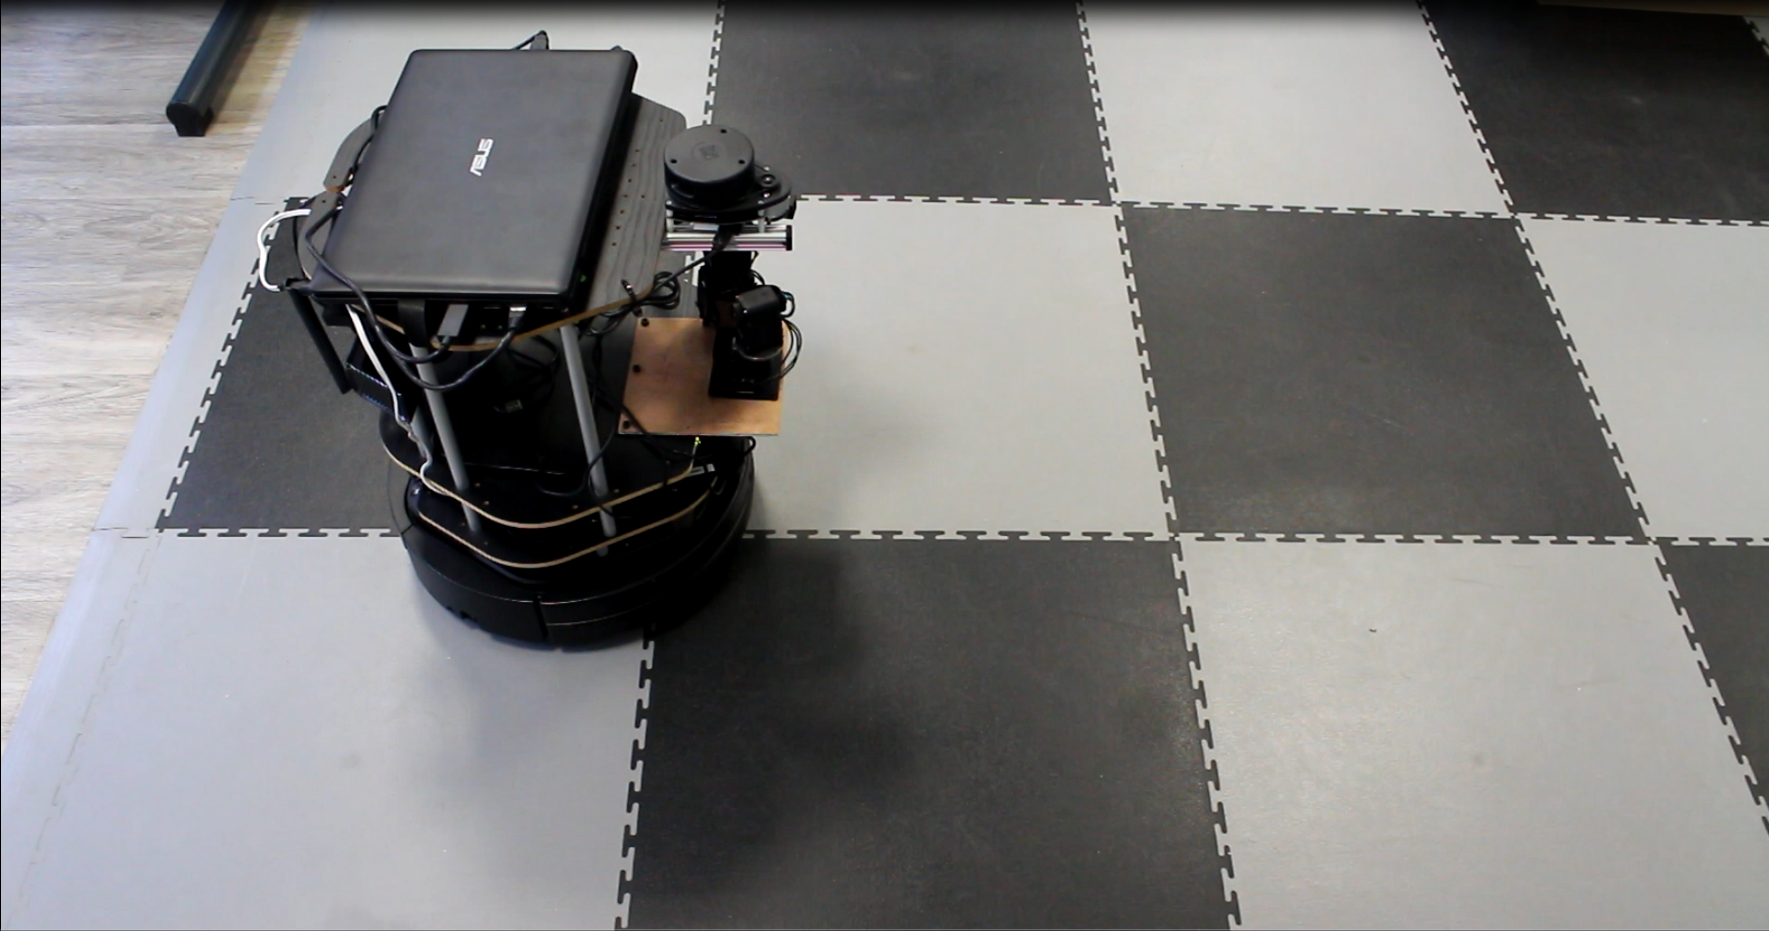
\includegraphics[width=7cm]{BackOdom2.png} }}
    \caption{Comparision between starting and ending positions}
    \label{fig:example}%
\end{figure}

We are now able to precisely move the robot in a straight line, and make it rotate accuratley. We can then try to change the angles and the number of loop to perform geometrical-shaped movement. 
\begin{figure}[H]
	\centering
	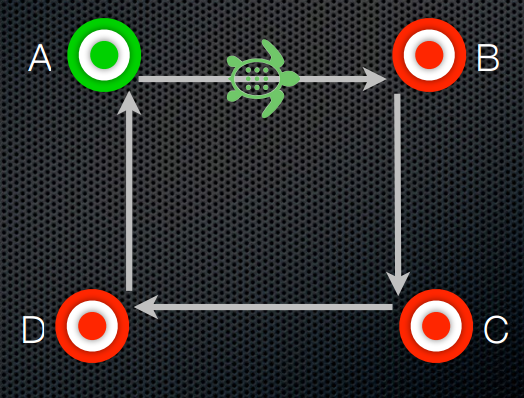
\includegraphics[height=8cm]{square.png}
	\caption{Square Movement}
	\label{fig: Square Movement}    
\end{figure}
For exemple, to make the robot moving squarly, we can set the rotation angle to 90° and the number of rotations to four. Our application's result is presented in \href{https://www.youtube.com/watch?v=kcxKbuMNRy4g}{this video}.

Previously, when were giving a distance to travel. An other way to control the robot is by giving a goal position, and use move\_base to move to this goal. This part, despite being provided is the Ros by example book, was somewhat complicated to understand. We did spend quite some time to understand the Quaternions. Although this subject looks interesting, we understood the basics only, enough to know that it is representing a position in a given space. We can then set this position as a waypoint for the robot to go. The second intresting part is the link between the Python code and Rviz. In fact, as the robot is at the center of its reference frame (the odometry frame), and the waypoint re choosen in the script, it is possible to place markers on the frame on Rviz, as shown below.

\begin{figure}[H]
	\centering
	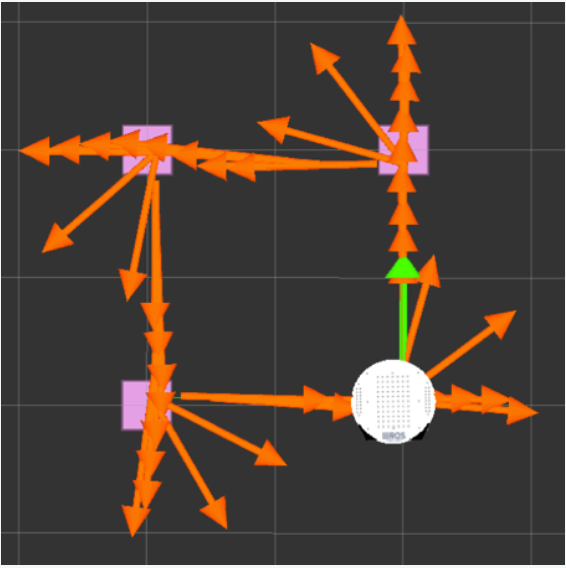
\includegraphics[height=8cm]{markers.png}
	\caption{Curve Movement}
	\label{fig: Markers}    
\end{figure} 

We did not work to much on the marker, as this is for display only, and we are here trying to get the basics of ROS. As speaking of basics, the TurtleBot in not only an old vaccum cleaner: it is a vaccum cleaner equipped with eyes.

\subsection{Adding and controlling sensors}
In this part, we will not talk about the internal sensors of the robot (cliff sensor, gyroscope, and others) but focus on the external sensors, and moslty on the RPLIDAR.
The TurtleBot comes equipped with a Kinect. As some former stutents used it previously with a strong calibration setting, we lost some time trying to make it work. In vain. After the hardware was changed, we had a bit of time left to spend on this part. We quickly used it with Rviz to see how the video is rendered, but we did not try to do our own application with it.
Instead, we focused on the RPLIDAR.As this sensor is not part of the robot when sell, we assume that either former students or professors ROSified it. And knowing the ease we had to use it, it was done greatly. The launch file provided by our professors allowed us to use it in a simple way, without having to remap the topics to the multiplxer. Here is this launch file: 

\launchexternal{remap_rplidar_minimal.launch}
All credits go to \href{https://github.com/roboticslab-fr}{Computer Vision for Robotics Laboratory}.

Using Rviz and a Joystick, we are then able to visualize the feedback given by the RPLIDAR while moving around the room. Below is shown a picture of the Rviz rendering: 

\begin{figure}[H]
	\centering
	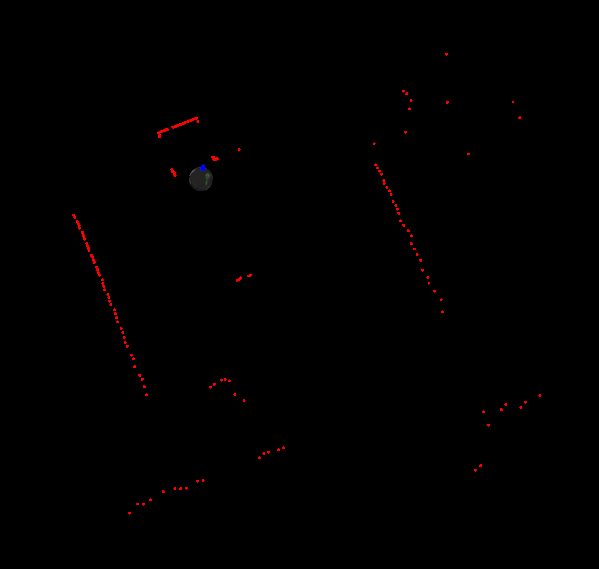
\includegraphics[height=8cm]{RPLIDAR.png}
	\caption{RPLIDAR data}
	\label{fig: RPLIDAR}    
\end{figure} 

As we are now able to use the RPLIDAR, we can try to perfom a mapping of the room.

\subsection{ACML and Gmapping}
In this section, we will use the RPLIDAR combined with the ROS package Gmapping to create a map of the laboratory.
In order to do so, several ROS commands should be used.

On the TurtleBot laptop: 
\begin{itemize}
  \item \textit{\$ roslaunch turtlebot\_le2i  remap\_rplidar\_minimal.launch}, being the mandatory minimal launch file
  \item \textit{\$ roslaunch rbx1\_nav gmapping\_demo.launch}, being a launch file provided with the ROS by example book, handling the mapping
  \item \textit{\$ roslaunch rbx1 \_nav joystick\_teleop.launch}, in order to move the robot around using the joystick
\end{itemize}

We then need to start Rviz on the workstation, as well as the usual bag file recording process:
\begin{itemize}
  \item \textit{\$ rosrun rviz rviz -d `rospack find rbx1\_nav`/gmapping.rvizh}, being a convenient Rviz configuration for this application
  \item \textit{\$ rosbag record -O map\_bag /scan /tf}, to record a bag with relevant topics and nodes.
\end{itemize}

Once the map appearing on Rviz is as expected by the user, the bag recodring process should be killed by doing Ctrl + C in the terminal window. 
The very last step is to extract the map from the bag file by using the following command: \textit{\$ rosrun map\_server map\_saver -f new\_map}. This will create the map `new\_map' in the current folder. This map is divided in two files: a yaml file, which is a configuration file, containing especially the starting position of the robot on the map; and a .pgm file being the rgaphical representation of the map. Here is our result:

\begin{figure}[H]
	\centering
	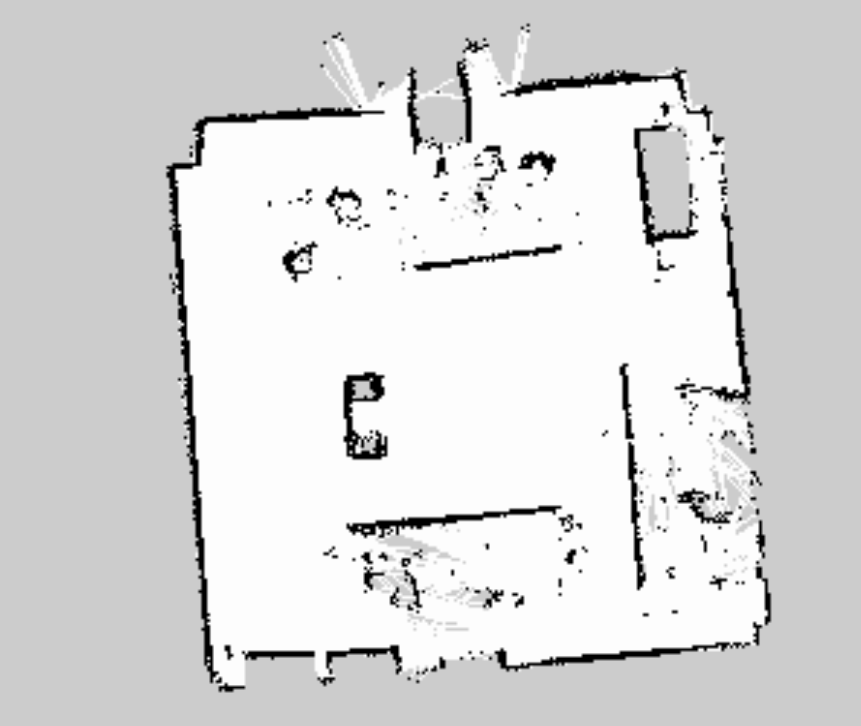
\includegraphics[height=8cm]{finalmap.png}
	\caption{Map of the laboratory}
	\label{fig: map}    
\end{figure} 

This map can be modified manually to correct any imprecision. As it is, the previously shown map can be used to drive the robot automatically from on point to another, using Rviz. The first step is to start the minimal file \textit{\$ roslaunch turtlebot\_le2i  remap\_rplidar\_minimal.launch} followed by the launch file \textit{\$ roslaunch rbx1\_nav tb\_demo\_amcl.launch map:=new\_map.yaml}, both on the TurtleBot laptop. Finally, we need Rviz on the workstation to visualize the map \textit{\$rosrun rviz rviz -d `rospack find rbx1\_nav`/nav\_test.rviz}. Then, on Rviz, a rough estimation of the robot on the map should be given. Once done, we can select a 2D Nav Goal as the goal for the robot to reach. And the Turtlebot will avoid known obtacle and perfom automatic pathfinding to reach the goal. 

\section{Merging TurtleBot and PhantomX Arm Pincher}

TODO
Previously, we learned the basics of ROS, going from simple movement to map creation and automated pathfinding. The next step is to try to bring something new to ROS, or at least to our own TurtleBot: a arm.
We produced a design to fix the PhantomX on the TurtleBot

\section{Challenges encountered}
Greatest challenge of all: we were not fortunate with the Hardware. We faced several malfunctions: 

\begin{itemize}
  \item The Kinect, which had to be replaced
  \item The TrutleBot battery, wich was failling also, crashing the robot for no appearing reasons. This malfunction did cost us several hours of our time
  \item The arduino board of the PhantomX, which crashed near the end of our project
  \item And finally (and again), the PhantomX Arm Pincher and its loose cables, resulting in time wasting to teak the cables until the Servo ID would be recognized.
\end{itemize}

These are the Hardware issues that we could not do anything about. but we also had to face challenges inherant to ourselves.
At first we had some difficulties to understand the combinasion of ROS and the SSH connection. We lost quite some time by putting the commands on the wrong computer. We then faced our lack of organization, forgetting to record some bag files, or not being rigourous with our method. We quickly learn to correct this, as from one week to another nothing was working anymore. 
It also took us some time to get use to the ROS methods used in Python. We do know the Python language, but its use in the specific domain being ROS requires some knowledge about the libraries and packages.
Finally, we were not using Rviz and Rqt-graph during the first half of our project. These are great tools to supervise the robot, but also to debug it. A lot of the time, a quick look at the Rqt-graph can tell you which node is not working as intended.

Overall, we improved our working method during the project, and were able to spend less and less time on our own mistakes by producing less of it. 

\section{Conclusion}

During this project, we put at use our knowledge of ROS acquired during the lessons. We were able to understand and modify Pythons scripts to move the robot, and we are now able to create basic ones by oursleves. From all our pratical our during these 9 weeks, we learn a lot about the theory( and strengthened the previously acquired one) , such as the management of the cmd\_vel multiplexer or the use of Rviz. We went from moving the robot ina straight line to automatic robot navigation in a previously set environnement. Our project is now finished, but the foundations laid down by the merging of the PhantomX Arm Pincher with the TurtleBot can be a solid base for future projects (Asynchronous control of the robot and the arm for example). This project really deepened our knowledge about ROS, but also regarding project managemend, teamwork and inter-team collaboration. 

\section{Appendix}
All our source code for the project, this report, and our defence can be found on \href{https://github.com/AntoineMerlet/Robotics}{Github} and on our open \href{https://drive.google.com/open?id=0B8c8pooKt7IPRXBxaTRpV3JIWFU}{Google Drive}.
All the lessons used for this project can be found \href{https://drive.google.com/open?id=0B8c8pooKt7IPTnRKSmtnVlMtTHc}{here}. We do not own any of it, all the credits goes to the author mentionned in each file.

Figures 1 \& 2 belongs to TrossenRobotics.
Figures 3, 5 \& 7 are taken from the ROS by example book.
All the other Figures were produced by our team.
\end{document} % DONE WITH DOCUMENT!


%https://www.generationrobots.com/fr/401271-turtlebot-2-robot-mobile-ros.html
